\documentclass[11pt,a4paper]{article}
\usepackage[utf8]{inputenc}
\usepackage[T1]{fontenc}
\usepackage{geometry}
\usepackage{hyperref}
\usepackage{listings}
\usepackage{xcolor}
\usepackage{booktabs}
\usepackage{array}
\usepackage{fancyhdr}
\usepackage{enumitem}
\usepackage{float}
\usepackage{mdframed}
\usepackage{tikz}
\usepackage{graphicx}
\usetikzlibrary{shapes,arrows,positioning,fit,backgrounds}

\geometry{margin=1in}

\definecolor{hydra-blue}{RGB}{5,32,73}
\definecolor{code-bg}{RGB}{248,248,248}
\definecolor{warning-bg}{RGB}{255,243,205}
\definecolor{success-bg}{RGB}{212,237,218}
\definecolor{info-bg}{RGB}{217,237,247}

\hypersetup{colorlinks=true,linkcolor=hydra-blue,urlcolor=blue}

\lstdefinestyle{bash}{backgroundcolor=\color{code-bg},basicstyle=\ttfamily\small,breaklines=true,frame=single,numbers=none}
\lstdefinestyle{js}{backgroundcolor=\color{code-bg},basicstyle=\ttfamily\small,breaklines=true,frame=single,numbers=left,language=Java}

\newmdenv[backgroundcolor=warning-bg,linewidth=0pt,innerleftmargin=10pt,innerrightmargin=10pt,innertopmargin=10pt,innerbottommargin=10pt]{warningbox}
\newmdenv[backgroundcolor=success-bg,linewidth=0pt,innerleftmargin=10pt,innerrightmargin=10pt,innertopmargin=10pt,innerbottommargin=10pt]{successbox}
\newmdenv[backgroundcolor=info-bg,linewidth=0pt,innerleftmargin=10pt,innerrightmargin=10pt,innertopmargin=10pt,innerbottommargin=10pt]{infobox}

\pagestyle{fancy}
\fancyhf{}
\fancyhead[L]{\textbf{Hydra Infrastructure}}
\fancyhead[R]{\textbf{Management Guide}}
\fancyfoot[C]{\thepage}
\setlength{\headheight}{14pt}

\title{\textbf{Hydra Infrastructure Management Guide}\\[0.5em]\large Student Container Platform Administration}
\author{Computer Science Department\\SUNY New Paltz}
\date{Last Updated: January 2025}

\begin{document}
\maketitle
\tableofcontents
\newpage

\section{System Overview}

Hydra is a containerized development platform providing persistent development environments for Computer Science students and faculty at SUNY New Paltz. The system uses SAML 2.0 Single Sign-On via Azure AD and Docker for container orchestration.

\subsection{Key Features}
\begin{itemize}
    \item \textbf{SSO Authentication:} Azure AD SAML 2.0 with automatic user provisioning
    \item \textbf{Persistent Containers:} One development environment per student with data persistence
    \item \textbf{Built-in Services:} VS Code (code-server), Jupyter Notebook, Docker-in-Docker
    \item \textbf{Dynamic Routing:} Traefik-based routing for custom web applications
    \item \textbf{Resource Management:} Per-container CPU and memory limits
    \item \textbf{Integration:} OpenWebUI (GPT) and n8n account management
\end{itemize}

\subsection{Access URLs}
\begin{table}[H]
\centering
\begin{tabular}{lll}
\toprule
\textbf{Service} & \textbf{URL} & \textbf{Description} \\
\midrule
Dashboard & \texttt{https://hydra.newpaltz.edu/dashboard} & Main user interface \\
OpenWebUI & \texttt{https://gpt.hydra.newpaltz.edu/} & AI chat interface \\
VS Code & \texttt{https://hydra.newpaltz.edu/students/\{user\}/vscode} & Browser IDE \\
Jupyter & \texttt{https://hydra.newpaltz.edu/students/\{user\}/jupyter} & Notebooks \\
\bottomrule
\end{tabular}
\end{table}

\section{System Architecture}

\subsection{Architecture Diagram}

\begin{center}
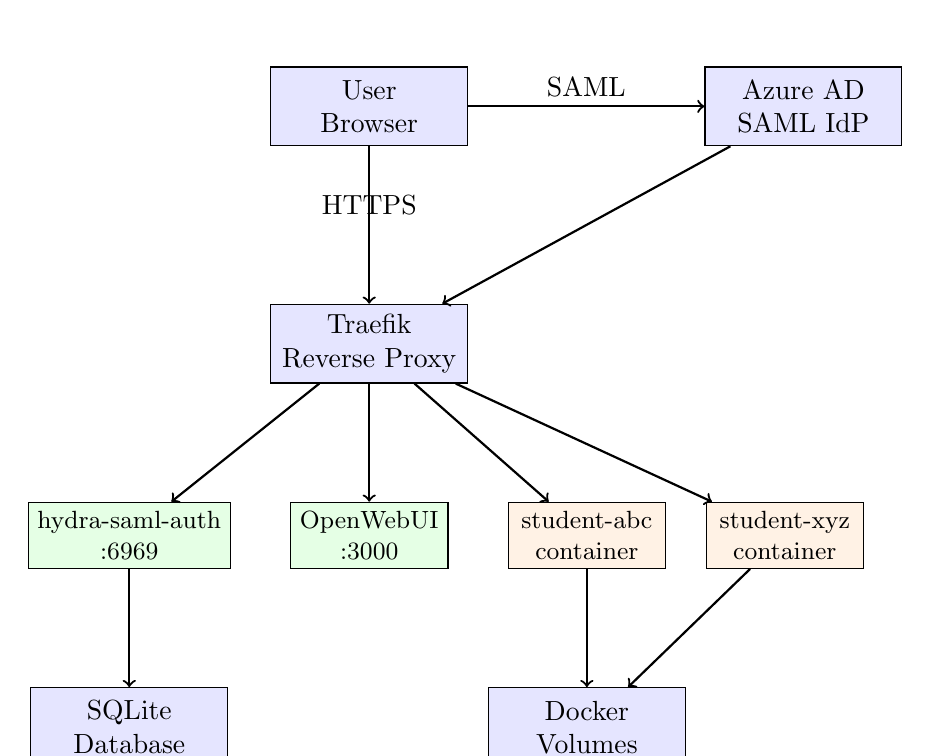
\begin{tikzpicture}[
    node distance=1.5cm,
    box/.style={rectangle, draw, fill=blue!10, minimum width=2.5cm, minimum height=1cm, align=center},
    service/.style={rectangle, draw, fill=green!10, minimum width=2cm, minimum height=0.8cm, align=center, font=\small},
    container/.style={rectangle, draw, fill=orange!10, minimum width=2cm, minimum height=0.8cm, align=center, font=\small},
    arrow/.style={->, thick}
]

% External
\node[box] (user) {User\\Browser};
\node[box, right=3cm of user] (azure) {Azure AD\\SAML IdP};

% Traefik
\node[box, below=2cm of user] (traefik) {Traefik\\Reverse Proxy};

% Services
\node[service, below left=1.5cm and 0.5cm of traefik] (hydra) {hydra-saml-auth\\:6969};
\node[service, below=1.5cm of traefik] (webui) {OpenWebUI\\:3000};

% Student containers
\node[container, below right=1.5cm and 0.5cm of traefik] (student1) {student-abc\\container};
\node[container, right=0.5cm of student1] (student2) {student-xyz\\container};

% Storage
\node[box, below=1.5cm of hydra] (db) {SQLite\\Database};
\node[box, below=1.5cm of student1] (volumes) {Docker\\Volumes};

% Arrows
\draw[arrow] (user) -- node[above] {HTTPS} (traefik);
\draw[arrow] (user) -- node[above] {SAML} (azure);
\draw[arrow] (azure) -- (traefik);
\draw[arrow] (traefik) -- (hydra);
\draw[arrow] (traefik) -- (webui);
\draw[arrow] (traefik) -- (student1);
\draw[arrow] (traefik) -- (student2);
\draw[arrow] (hydra) -- (db);
\draw[arrow] (student1) -- (volumes);
\draw[arrow] (student2) -- (volumes);

\end{tikzpicture}
\end{center}

\subsection{Component Overview}

\begin{table}[H]
\centering
\begin{tabular}{llp{6cm}}
\toprule
\textbf{Component} & \textbf{Port} & \textbf{Description} \\
\midrule
Traefik & 80, 443 & Reverse proxy, TLS termination, routing \\
hydra-saml-auth & 6969 & SAML auth, dashboard, container management \\
OpenWebUI & 3000 & AI chat interface (Ollama frontend) \\
Student Containers & Dynamic & Per-user development environments \\
\bottomrule
\end{tabular}
\end{table}

\subsection{Network Architecture}

Student containers operate on an isolated Docker network (\texttt{hydra\_students\_net}) with:
\begin{itemize}
    \item No direct internet access (configurable)
    \item Internal DNS resolution
    \item Traefik-mediated external access via ForwardAuth
\end{itemize}

\section{Authentication System}

\subsection{SAML 2.0 SSO Flow}

\begin{center}
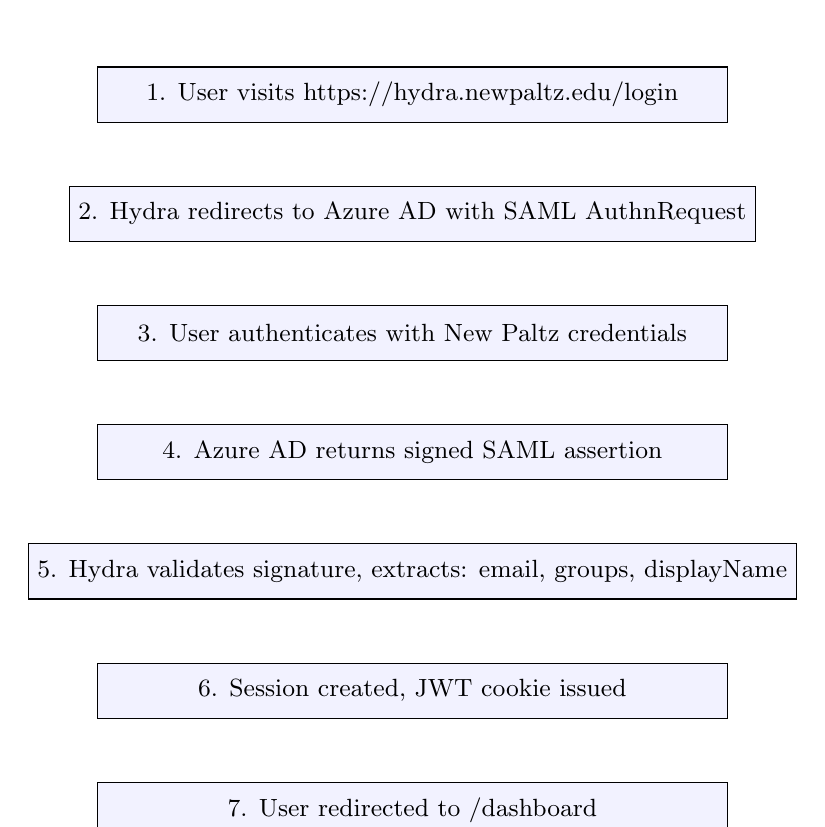
\begin{tikzpicture}[
    node distance=0.8cm,
    stepbox/.style={rectangle, draw, fill=blue!5, minimum width=8cm, minimum height=0.7cm, align=left, font=\small}
]
\node[stepbox] (s1) {1. User visits https://hydra.newpaltz.edu/login};
\node[stepbox, below=of s1] (s2) {2. Hydra redirects to Azure AD with SAML AuthnRequest};
\node[stepbox, below=of s2] (s3) {3. User authenticates with New Paltz credentials};
\node[stepbox, below=of s3] (s4) {4. Azure AD returns signed SAML assertion};
\node[stepbox, below=of s4] (s5) {5. Hydra validates signature, extracts: email, groups, displayName};
\node[stepbox, below=of s5] (s6) {6. Session created, JWT cookie issued};
\node[stepbox, below=of s6] (s7) {7. User redirected to /dashboard};
\end{tikzpicture}
\end{center}

\subsection{Session Management}

Sessions are managed via:
\begin{itemize}
    \item \textbf{Express Session:} Server-side session storage in SQLite
    \item \textbf{JWT Cookie:} Site-wide authentication cookie for cross-service SSO
    \item \textbf{JWKS Endpoint:} Public key endpoint for JWT verification by other services
\end{itemize}

\begin{infobox}
\textbf{JWT Configuration:}
\begin{itemize}
    \item TTL: Configurable via \texttt{JWT\_TTL\_SECONDS} (default: 86400)
    \item Algorithm: RS256
    \item Cookie Domain: \texttt{.newpaltz.edu}
\end{itemize}
\end{infobox}

\section{Container System}

\subsection{Student Container Features}

Each student receives a single persistent container with:

\begin{table}[H]
\centering
\begin{tabular}{lp{8cm}}
\toprule
\textbf{Feature} & \textbf{Details} \\
\midrule
Node.js & Latest LTS via nvm \\
Python & 3.11+ with pip, venv, Jupyter \\
Java & OpenJDK 21 \\
Docker & Full Docker-in-Docker support (privileged mode) \\
VS Code & code-server browser IDE \\
Jupyter & Notebook and JupyterLab \\
Tools & Git, curl, wget, build-essential, etc. \\
\bottomrule
\end{tabular}
\end{table}

\subsection{Resource Limits}

\begin{table}[H]
\centering
\begin{tabular}{ll}
\toprule
\textbf{Resource} & \textbf{Limit} \\
\midrule
RAM & 4GB per container \\
CPU & 2 cores per container \\
Storage & Unlimited (host disk limited) \\
\bottomrule
\end{tabular}
\end{table}

\begin{warningbox}
\textbf{Security Note:} Student containers run in privileged mode to support Docker-in-Docker. This grants elevated access. Monitor for abuse and consider disabling for untrusted users.
\end{warningbox}

\subsection{Port Routing}

Students can expose web applications through custom routes:

\begin{itemize}
    \item Default routes: \texttt{/students/\{username\}/vscode}, \texttt{/students/\{username\}/jupyter}
    \item Custom routes added via dashboard UI
    \item Reserved ports: 8443 (code-server), 8888 (Jupyter)
    \item All routes protected by ForwardAuth
\end{itemize}

\section{File Structure}

\begin{lstlisting}[style=bash]
hydra-saml-auth/
|-- index.js              # Main entry: SAML, JWT/JWKS, routes, WebSocket
|-- db.js                 # SQLite database initialization
|-- routes/
|   |-- containers.js     # Container lifecycle, services, ports, logs
|   |-- webui-api.js      # OpenWebUI account proxy
|   |-- n8n-api.js        # n8n account management
|   |-- servers-api.js    # Cluster status endpoints
|   |-- admin.js          # Admin panel routes
|-- services/
|   |-- activity-logger.js    # Activity tracking
|   |-- email-notifications.js # Email alerts
|-- views/                # EJS templates
|-- student-container/
|   |-- Dockerfile        # Ubuntu 22.04 + dev tools
|   |-- supervisord.conf  # Process manager config
|   |-- entrypoint.sh     # Container startup
|-- docker-compose.yaml   # Production stack
|-- docs/                 # Documentation
\end{lstlisting}

\section{Common Operations}

\subsection{View Running Containers}
\begin{lstlisting}[style=bash]
docker ps --filter "name=student-"
\end{lstlisting}

\subsection{Access Container Shell}
\begin{lstlisting}[style=bash]
docker exec -it student-<username> /bin/bash
\end{lstlisting}

\subsection{View Container Logs}
\begin{lstlisting}[style=bash]
docker logs -f student-<username> --tail=100
\end{lstlisting}

\subsection{Restart a Container}
\begin{lstlisting}[style=bash]
docker restart student-<username>
\end{lstlisting}

\subsection{Remove a Stuck Container}
\begin{lstlisting}[style=bash]
docker rm -f student-<username>
\end{lstlisting}

\subsection{Rebuild Student Container Image}
\begin{lstlisting}[style=bash]
cd student-container
docker build -t hydra-student-container:latest .
\end{lstlisting}

\begin{infobox}
\textbf{Note:} Students with existing containers must recreate them to use updated images.
\end{infobox}

\section{Service Management}

\subsection{Restart Main Service}
\begin{lstlisting}[style=bash]
docker compose restart hydra-saml-auth
\end{lstlisting}

\subsection{Rebuild and Redeploy}
\begin{lstlisting}[style=bash]
docker compose build hydra-saml-auth
docker compose up -d hydra-saml-auth
\end{lstlisting}

\subsection{View Service Logs}
\begin{lstlisting}[style=bash]
docker compose logs -f hydra-saml-auth
\end{lstlisting}

\subsection{Check Traefik Routing}
\begin{lstlisting}[style=bash]
docker compose logs traefik | grep -i error
curl -I https://hydra.newpaltz.edu/
\end{lstlisting}

\section{Troubleshooting}

\subsection{Authentication Issues}

\begin{table}[H]
\centering
\begin{tabular}{lp{8cm}}
\toprule
\textbf{Symptom} & \textbf{Solution} \\
\midrule
SAML assertion invalid & Verify \texttt{METADATA\_URL} and \texttt{SAML\_SP\_ENTITY\_ID} match Azure config exactly \\
Cookie not set & Check \texttt{COOKIE\_DOMAIN}, ensure HTTPS, check browser settings \\
JWT verification fails & Verify JWKS endpoint accessible, check key rotation \\
\bottomrule
\end{tabular}
\end{table}

\subsection{Container Issues}

\begin{table}[H]
\centering
\begin{tabular}{lp{8cm}}
\toprule
\textbf{Symptom} & \textbf{Solution} \\
\midrule
Container won't initialize & Verify \texttt{hydra-student-container:latest} image exists \\
Container 404 & Check container is on \texttt{hydra\_students\_net}, Traefik running \\
Service won't start & Check supervisord logs inside container \\
Port routing fails & Verify port not reserved (8443, 8888) and not in use \\
\bottomrule
\end{tabular}
\end{table}

\subsection{Service-Specific Issues}

\begin{itemize}
    \item \textbf{VS Code not loading:} Check code-server process, ForwardAuth working
    \item \textbf{Jupyter issues:} Verify \texttt{NotebookApp.base\_url} setting
    \item \textbf{Docker-in-Docker fails:} Container must have privileged mode
    \item \textbf{Files not persisting:} Only \texttt{/home/student/} is persisted
\end{itemize}

\section{Backup and Recovery}

\subsection{Database Backup}
\begin{lstlisting}[style=bash]
# Backup SQLite database
sqlite3 /app/data/webui.db ".backup '/backups/hydra-$(date +%Y%m%d).db'"

# Automated daily backup (add to crontab)
0 2 * * * sqlite3 /app/data/webui.db ".backup '/backups/hydra-$(date +\%Y\%m\%d).db'"
\end{lstlisting}

\subsection{Volume Backup}
\begin{lstlisting}[style=bash]
# List student volumes
docker volume ls | grep student-

# Backup a volume
docker run --rm -v student-<user>-data:/data -v $(pwd):/backup \
    alpine tar cvf /backup/student-<user>-backup.tar /data
\end{lstlisting}

\section{Environment Configuration}

\subsection{Required Variables}
\begin{table}[H]
\centering
\begin{tabular}{lp{7cm}}
\toprule
\textbf{Variable} & \textbf{Description} \\
\midrule
\texttt{BASE\_URL} & External URL (https://hydra.newpaltz.edu) \\
\texttt{METADATA\_URL} & Azure AD federation metadata URL \\
\texttt{SAML\_SP\_ENTITY\_ID} & SP Entity ID (must match Azure exactly) \\
\texttt{COOKIE\_DOMAIN} & Cookie scope (.newpaltz.edu) \\
\texttt{PORT} & Service port (default: 6969) \\
\texttt{DB\_PATH} & Database path (/app/data/webui.db) \\
\bottomrule
\end{tabular}
\end{table}

\subsection{Optional Variables}
\begin{table}[H]
\centering
\begin{tabular}{lp{7cm}}
\toprule
\textbf{Variable} & \textbf{Description} \\
\midrule
\texttt{PUBLIC\_STUDENTS\_BASE} & Student URL base (https://hydra.newpaltz.edu/students) \\
\texttt{JWT\_TTL\_SECONDS} & JWT token lifetime \\
\texttt{JWT\_PRIVATE\_KEY\_FILE} & Path to JWT signing key \\
\texttt{JWT\_PUBLIC\_KEY\_FILE} & Path to JWT verification key \\
\bottomrule
\end{tabular}
\end{table}

\section{References}

\begin{itemize}
    \item Docker Documentation: \url{https://docs.docker.com/}
    \item Traefik Documentation: \url{https://doc.traefik.io/traefik/}
    \item SAML 2.0 Specification: \url{https://docs.oasis-open.org/security/saml/v2.0/}
    \item Azure AD SAML: \url{https://docs.microsoft.com/en-us/azure/active-directory/develop/single-sign-on-saml-protocol}
    \item code-server: \url{https://coder.com/docs/code-server/latest}
    \item Jupyter: \url{https://jupyter.org/documentation}
\end{itemize}

\end{document}
